\documentclass{article}
\usepackage[hyphens]{url}
\usepackage{mathtools}
\usepackage{amsmath}
\usepackage{listings}
\usepackage{graphicx}
\usepackage[margin=1in]{geometry}
\usepackage{float}
\floatstyle{boxed}
\restylefloat{figure}
\lstset{breaklines=true}
\begin{document}


\title{CS595 Intro to Web Science, Assignment \#3}
\author{Valentina Neblitt-Jones}
\date{October 5, 2013}
\maketitle

\section*{Question 1}

Download the 1000 URIs from assignment \#2. ``curl'', ``wget'', or ``lynx'' are all good candidate programs to use. We just want the raw HTML, not the images, stylesheets, etc.

from the command line:

\% curl http://www.cnn.com/  \textgreater  www.cnn.com

\% wget -O www.cnn.com http://www.cnn.com

\% lynx -source http://www.cnn.com/ \textgreater www.cnn.com

``www.cnn.com'' is just an example output file name, keep in mind that the shell will not like some of the characters that can occur in the URIs (e.g., ``?'', ``\&''). You might want to hash the URIs, like:

\% echo -n``http://www.cs.odu.edu/show\_features.shtml?72'' | md5
41d5f125d13b4bb554e6e31b6b591eeb

(``md5sum'' on some machines; note the ``-n'' in echo -- this removes the trailing newlines.)

Now use a tool to remove (most) of the HTML markup. ``lynx'' will do a fair job:

\% lynx -dump -force\_html www.cnn.com \textgreater www.cnn.com.processed

Use another (better) tool if you know of one. Keep both files for each URI (i.e., raw HTML and processed).

\subsection*{Answer to Question 1}

I separated the task into two scripts - one that downloads the URIs (Figure \ref{downloadURI}) and then one that strips the HTML markup (Figure \ref{rmMarkup}). Figure \ref{before} shows a file before removing HTML markup and Figure \ref{after} shows the file after removing HTML markup. Additionally, a finding aid was developed in order to match up the md5 with the URI (Figure \ref{findingaid}).

\begin{figure}[H]
\centering
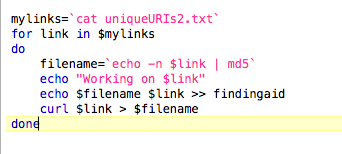
\includegraphics{q1/downloadURI}
\caption{Shell Script to Download URIs}
\label{downloadURI}
\end{figure}

\begin{figure}[H]
\centering
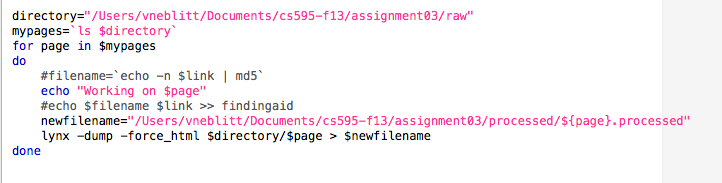
\includegraphics[scale=0.50]{q1/rmMarkupURI}
\caption{Shell Script to Remove Markup}
\label{rmMarkup}
\end{figure}

\begin{figure}[H]
\centering
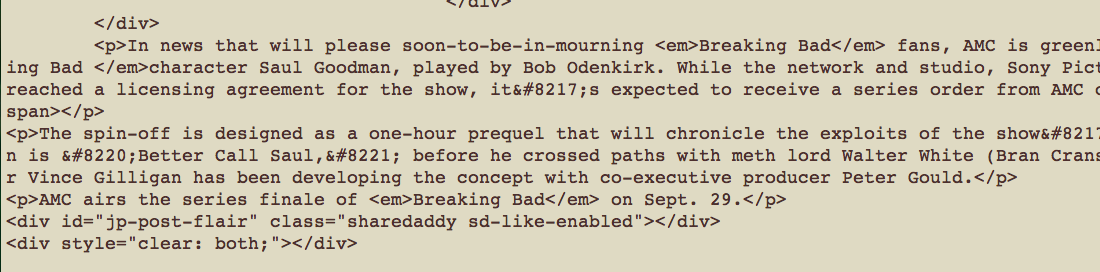
\includegraphics[scale=0.40]{q1/beforermmarkup}
\caption{File Before Removing Markup}
\label{before}
\end{figure}

\begin{figure}[H]
\centering
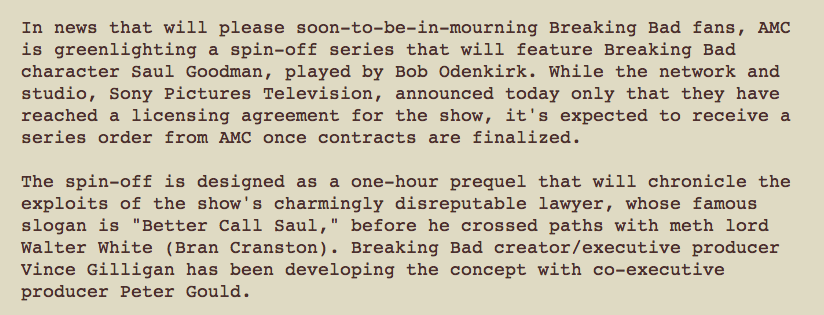
\includegraphics[scale=0.50]{q1/afterrmmarkup}
\caption{File After Removing Markup}
\label{after}
\end{figure}

\begin{figure}[H]
\centering
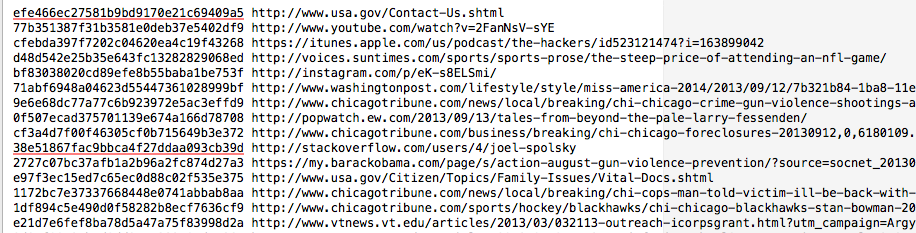
\includegraphics[scale=0.50]{q1/findingaid}
\caption{Finding Aid}
\label{findingaid}
\end{figure}

\newpage

\section*{Question 2}

Chose a query term (e.g., ``shadow'') that is not a not a stop words (see week 4 slides) and not HTML markup from step 1 (e.g., ``http'') that matches at least 10 documents (hint: use ``grep'' on the processed files). If the term is present in more than 10 documents, choose any 10 from your list. (If you do not end up with a list of 10 URIs, you've done something wrong).

As per the example in the week 4 slides, computer the TFIDF values for the term in each of the 10 documents and create a table with the TF, IDF, and TFIDF values, as well as the corresponding URIs. The URIs will be ranked in decreasing order by the TFIDF values. For example:

\begin{table}[!h]
\centering
\caption{10 Hits for the term ``shadow'', ranked by TFIDF}
\begin{tabular}{c c c c}
\hline
TFIDF & TF & IDF & URI \\
\hline
\hline
0.150 & 0.014 & 10.680 & http://foo.com \\
0.085 & 0.008 & 10.680 & http://bar.com \\
\hline
\end{tabular}
\end{table}

You can use Google or Bing for the DF estimation. To count the number of words in the processed document (i.e., the denominator for TF),  you can use ``wc'':

\% wc -w www.cnn.com.processed

2370 www.cnn.com.processed

It won't be completely accurate, but it will probably be consistently inaccurate across all files. You can use more accurate methods if you'd like.

Don't forget the log base 2 for IDF, and mind your significant digits!

\subsection*{Answer to Question 2}

I used the term ``budget'' since that topic is currently affecting over half of the income coming into my household right now. To determine the term frequency, I needed to compare the number of times the term appeared in the document divided by the number of words total in the document. But first to find documents with the term. To determine the goodness of using ``budget'', I used grep to determine how many documents contained the term.

\begin{verbatim}
grep -l budget * > ../q2/pagescontainbudget
\end{verbatim}

This produced a file that contained 92 results so ``budget'' turned out to be a good term to use. Table \ref{tfcalculation} shows the results of finding the term ``budget'' in each file using grep, using wc -w for each file to get total word count and dividing the former by the latter. \\

\begin{table}[h!]
\centering
\caption{Term Frequency Calculation for ``budget'', ranked by TF}
\begin{tabular}{p{8cm}c c c }
\hline
URI & Term Count & Word Count & TF \\
\hline
\hline
\url{http://www.usa.gov/Citizen/Topics/Health/Food.shtml#Eating_on_a_Budget} & 4 & 1315 & 0.0030 \\
\url{http://www.vtnews.vt.edu/articles/2013/06/060313-bov-overview.html} & 5 & 1665 & 0.0030 \\
\url{http://thehill.com/blogs/floor-action/senate/295759-reid-proposes-new-background-check-requirement-for-explosives}	& 5 & 2054 & 0.0024 \\
\url{http://news.harvard.edu/gazette/story/2013/09/managing-a-seismic-shift/} & 6 & 2499	& 0.0024 \\
\url{http://www.huffingtonpost.com/2013/08/14/sequestration-cuts_n_3749432.html} & 21 & 11950 & 0.0018 \\
\url{http://www.washingtonpost.com/politics/from-newtown-to-navy-yard-unpredictable-calamities-upend-obamas-second-term/2013/09/16/3df366a6-1f04-11e3-8459-657e0c72fec8_story.html} & 5 & 3511 & 0.0014 \\
\url{http://www.tampabay.com/blogs/media/eric-deggans-to-leave-tampa-bay-times-for-job-as-nprs-first-tv-critic/2134332} & 4 & 3985 & 0.0010 \\
\url{http://maddowblog.msnbc.com/_news/2013/07/12/19436633-watching-marco-rubio-go-around-the-bend?lite} & 5 & 6017 & 0.0008 \\
\url{http://www.washingtoncitypaper.com/articles/44734/shadow-of-a-doubt-dc-statehood-activists/} & 7 & 9556 & 0.0007 \\
\url{http://www.huffingtonpost.com/2013/08/19/head-start-cuts-services\_n\_3779210.html?1376925983} & 4 & 6053 & 0.0007 \\
\hline
\end{tabular}
\label{tfcalculation}
\end{table}

I decided to use Google in the DF estimation. I looked up ``how many documents has google indexed'' in Google (Figure \ref{googlesize}) and chose the result for World Wide Web Size \url{http://www.worldwidewebsize.com/}. From Figure \ref{googlesizegraph}, you can see that it is estimated at 44 billion web pages. Furthermore, searching Google for the term ``budget'' yields 636,000,000 web pages (Figure \ref{budgetpages}).

\begin{verbatim}
Total pages in corpus = 44,000,000,000
Total pages in corpus with the term "budget" = 636,000,000
Total pages in corpus / total pages with the term = 69.1824
\end{verbatim}
$IDF(budget)= \log_2 69.1824 = 6.1123$ \\

Table \ref{tfidfcalculation} shows the results of calculations from Table \ref{tfcalculation} combined with the IDF calculations above.

\begin{figure}[H]
\centering
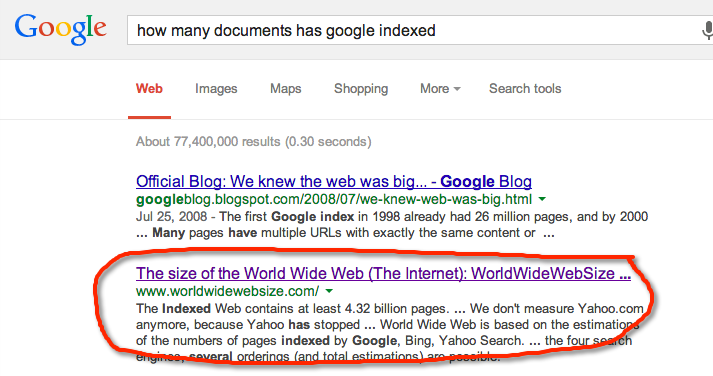
\includegraphics[scale=0.50]{q2/findinggooglesizecollection}
\caption{Finding the Size of Google's Collection}
\label{googlesize}
\end{figure}

\begin{figure}[H]
\centering
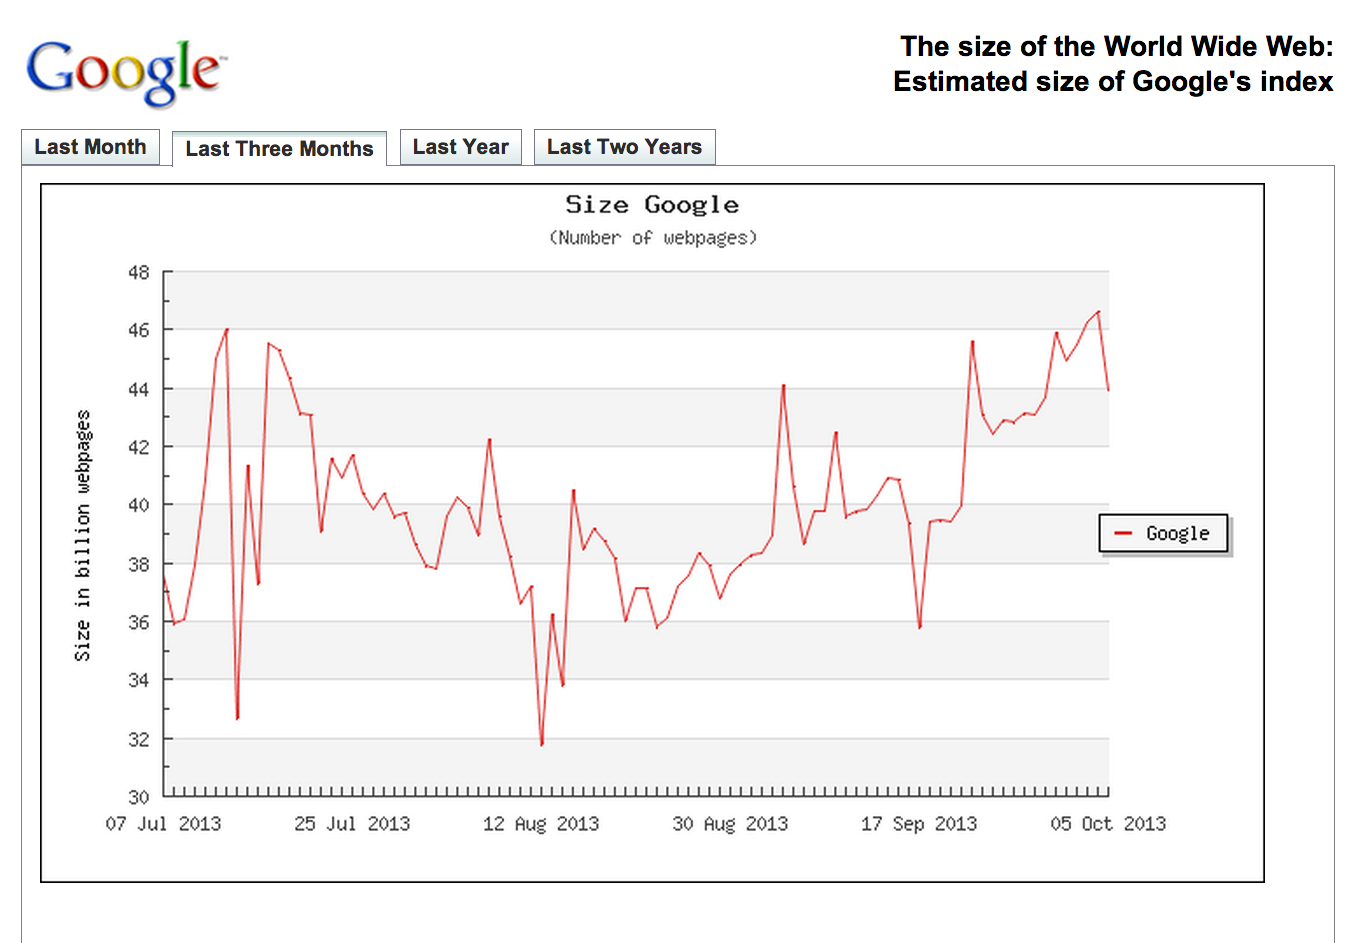
\includegraphics[scale=0.25]{q2/sizeofgooglecollection}
\caption{Size of Google's Collection}
\label{googlesizegraph}
\end{figure}

\begin{figure}[H]
\centering

\includegraphics[scale=0.50]{q2/docswithterm}
\caption{Pages with the Term ``Budget''}
\label{budgetpages}
\end{figure}

\begin{table}[!h]
\centering
\caption{10 Hits for the term ``budget'', ranked by TFIDF}
\begin{tabular}{c c c p{10cm}}
\hline
TFIDF & TF & IDF & URI \\
\hline
\hline
0.0186 & 0.0030 & 6.1123 & \url{http://www.usa.gov/Citizen/Topics/Health/Food.shtml#Eating_on_a_Budget} \\
0.0184 & 0.0030 & 6.1123 & \url{http://www.vtnews.vt.edu/articles/2013/06/060313-bov-overview.html} \\
0.0149 & 0.0024 & 6.1123 & \url{http://thehill.com/blogs/floor-action/senate/295759-reid-proposes-new-background-check-requirement-for-explosives} \\
0.0147 & 0.0024 & 6.1123 & \url{http://news.harvard.edu/gazette/story/2013/09/managing-a-seismic-shift} \\
0.0107 & 0.0018 & 6.1123 & \url{http://www.huffingtonpost.com/2013/08/14/sequestration-cuts_n_3749432.html} \\
0.0087 & 0.0014 & 6.1123 & \url{http://www.washingtonpost.com/politics/from-newtown-to-navy-yard-unpredictable-calamities-upend-obamas-second-term/2013/09/16/3df366a6-1f04-11e3-8459-657e0c72fec8_story.html} \\
0.0061 & 0.0010 & 6.1123 & \url{http://www.tampabay.com/blogs/media/eric-deggans-to-leave-tampa-bay-times-for-job-as-nprs-first-tv-critic/2134332} \\
0.0051 & 0.0008 & 6.1123 & \url{http://maddowblog.msnbc.com/_news/2013/07/12/19436633-watching-marco-rubio-go-around-the-bend?lite} \\
0.0045 & 0.0007 & 6.1123 & \url{http://www.washingtoncitypaper.com/articles/44734/shadow-of-a-doubt-dc-statehood-activists/} \\
0.0040 & 0.0007 & 6.1123 & \url{http://www.huffingtonpost.com/2013/08/19/head-start-cuts-services_n_3779210.html?1376925983} \\
\hline
\end{tabular}
\label{tfidfcalculation}
\end{table}

\clearpage

\section*{Question 3}

Now rank the same 10 URIs from question \#2, but this time by their PageRank. Use any of the free PR estimators on the web, such as:

http://www.prchecker.info/check\_page\_rank.php

http://www.seocentro.com/tools/search-engines/pagerank.html

http://www.checkpagerank.net

If you use these tools, you'll have to do so by hand (they have anti-bot captchas), but there is only 10. Normalize the values they give you to be from 0 to 1.0. Use the same tool on all 10 (again, consistency is more important than accuracy).

Create a table similar to Table 1.

\begin{table}[!h]
\centering
\caption{10 Hits for the term ``shadow'', ranked by PageRank}
\begin{tabular}{c p{10cm}}
\hline
PageRank & URI \\
\hline
\hline
0.9 & \url{http://foo.html} \\
0.5 & \url{http://bar.html} \\
\hline
\end{tabular}
\end{table}

\subsection*{Answer to Question 3}

I chose the first PageRank checker on the list \url{http://www.prchecker.info/check_page_rank.php}. Only one of my pages had a rank - a government web site (Figure \ref{prsuccess}). It was disappointing to not see a variety of ranks. Nine URIs got an N/A as a result (Figure \ref{unsuccessful}). The site offered the following reasons for why PageRank was not available:

\begin{enumerate}
\item The web page is new and not yet indexed
\item The web page is indexed but not yet ranked
\item The web page is indexed by Google, but recognized as a supplemental result
\item The web page or whole web site is banned by Google
\end{enumerate}

I think \#1 and \#2 are more likely reasons than \#3 and \#4 for why PageRank is not available for these pages. Of the ones with no rank, three are from September, three are from August, and the remaining ones are from July or earlier. These dates are not surprising since these URIs were extracted from recent tweets and tweeters are likely to reference more recent material. The age of these URIs should be enough time for them to be indexed, but not necessarily ranked. There does not appear to be a relationship between having a PageRank or even having a higher PageRank and the TFIDF value. Even though the usa.gov web page has the highest TFIDF and is the only one with a PageRank value, the next highest TFIDF value is not significantly lower than the usa.gov page, but does not have PageRank available.

\begin{figure}[H]
\centering
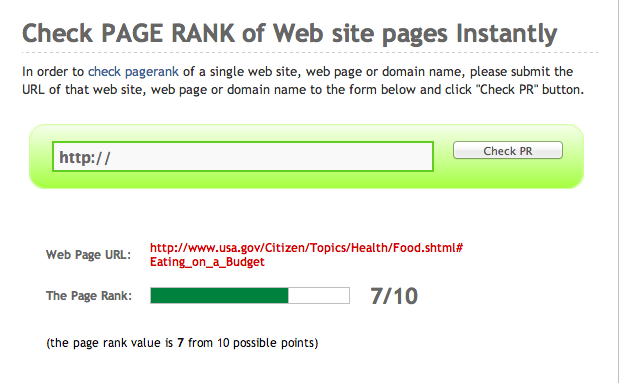
\includegraphics[scale=0.50]{q3/pagerankchecker}
\caption{Successful PageRank Obtained}
\label{prsuccess}
\end{figure}

\begin{figure}[H]
\centering
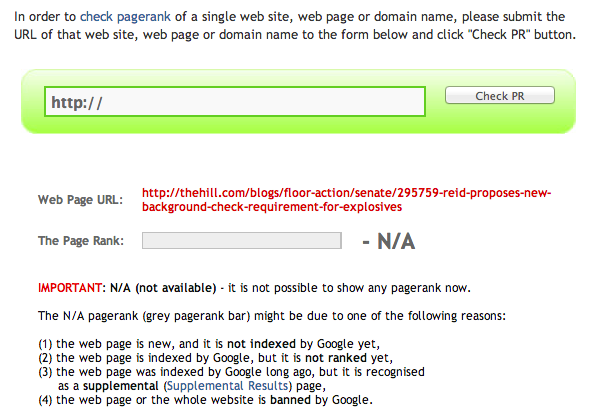
\includegraphics[scale=0.50]{q3/pagerankna}
\caption{No PageRank Obtained}
\label{unsuccessful}
\end{figure}

\begin{table}[!h]
\centering
\caption{10 Hits for the term ``budget'', ranked by PageRank}
\begin{tabular}{c p{10cm}}
\hline
PageRank & URI \\
\hline
\hline
0.7 & \url{http://www.usa.gov/Citizen/Topics/Health/Food.shtml#Eating_on_a_Budget} \\
0.0 & \url{http://www.vtnews.vt.edu/articles/2013/06/060313-bov-overview.html} \\
0.0 & \url{http://thehill.com/blogs/floor-action/senate/295759-reid-proposes-new-background-check-requirement-for-explosives} \\
0.0 & \url{http://news.harvard.edu/gazette/story/2013/09/managing-a-seismic-shift} \\
0.0 & \url{http://www.huffingtonpost.com/2013/08/14/sequestration-cuts_n_3749432.html} \\
0.0 & \url{http://www.washingtonpost.com/politics/from-newtown-to-navy-yard-unpredictable-calamities-upend-obamas-second-term/2013/09/16/3df366a6-1f04-11e3-8459-657e0c72fec8_story.html} \\
0.0 & \url{http://www.tampabay.com/blogs/media/eric-deggans-to-leave-tampa-bay-times-for-job-as-nprs-first-tv-critic/2134332} \\
0.0 & \url{http://maddowblog.msnbc.com/_news/2013/07/12/19436633-watching-marco-rubio-go-around-the-bend?lite} \\
0.0 & \url{http://www.washingtoncitypaper.com/articles/44734/shadow-of-a-doubt-dc-statehood-activists/} \\
0.0 & \url{http://www.huffingtonpost.com/2013/08/19/head-start-cuts-services_n_3779210.html?1376925983} \\
\hline
\end{tabular}
\end{table}

\clearpage
\section*{Question 4 - Extra Credit}

Compute the Kendall Tau\_b score for both lists (use ``b'' because there will likely be tie values in the rankings). Report both the Tau value and the ``p'' value.

See:

http://stackoverflow.com/questions/2557863/measures-of-association-in-r-kendalls-tau-b-and-tau-c

http://en.wikipedia.org/wiki/Kendall\_tau\_rank\_correlation\_coefficient\#Tau-b

http://en.wikipedia.org/wiki/Correlation\_and\_dependence

\subsection*{Answer to Question 4}

Not attempted.

\end{document}